\documentclass{article}
%\usepackage[T1,T2A]{fontenc}
\usepackage[utf8]{inputenc}
\usepackage[english,russian]{babel}
\usepackage{amsmath}
\usepackage{amssymb}
\usepackage{tikz}
\usepackage{enumitem}
\usepackage{graphicx}
\usepackage{multicol}

\usepackage{wrapfig}
\graphicspath{ {./pic/} }

\usepackage{hyperref}
\hypersetup{
    colorlinks=true,
    linkcolor=black,
    filecolor=magenta,      
    urlcolor=cyan,
}

% black text on white background
\usepackage{xcolor}
\usepackage{pagecolor}
\usepackage{mdframed}
\pagecolor{white}
\color{black}

% better font
\usepackage[defaultsans]{droidsans}
\renewcommand{\sfdefault}{ptm}
%\usepackage[T1]{fontenc}


\usepackage[a4paper]{geometry}
\usepackage{filecontents, pgffor}

% Copyright 2017 Sergei Tikhomirov, MIT License
% https://github.com/s-tikhomirov/solidity-latex-highlighting/

\usepackage{listings, xcolor}

\definecolor{verylightgray}{rgb}{.97,.97,.97}

\lstdefinelanguage{Solidity}{
	keywords=[1]{anonymous, assembly, assert, balance, break, call, callcode, case, catch, class, constant, continue, contract, debugger, default, delegatecall, delete, do, else, event, export, external, false, finally, for, function, gas, if, implements, import, in, indexed, instanceof, interface, internal, is, length, library, log0, log1, log2, log3, log4, memory, modifier, new, payable, pragma, private, protected, public, pure, push, require, return, returns, revert, selfdestruct, send, storage, struct, suicide, super, switch, then, this, throw, transfer, true, try, typeof, using, value, view, while, with, addmod, ecrecover, keccak256, mulmod, ripemd160, sha256, sha3}, % generic keywords including crypto operations
	keywordstyle=[1]\color{blue}\bfseries,
	keywords=[2]{address, bool, byte, bytes, bytes1, bytes2, bytes3, bytes4, bytes5, bytes6, bytes7, bytes8, bytes9, bytes10, bytes11, bytes12, bytes13, bytes14, bytes15, bytes16, bytes17, bytes18, bytes19, bytes20, bytes21, bytes22, bytes23, bytes24, bytes25, bytes26, bytes27, bytes28, bytes29, bytes30, bytes31, bytes32, enum, int, int8, int16, int24, int32, int40, int48, int56, int64, int72, int80, int88, int96, int104, int112, int120, int128, int136, int144, int152, int160, int168, int176, int184, int192, int200, int208, int216, int224, int232, int240, int248, int256, mapping, string, uint, uint8, uint16, uint24, uint32, uint40, uint48, uint56, uint64, uint72, uint80, uint88, uint96, uint104, uint112, uint120, uint128, uint136, uint144, uint152, uint160, uint168, uint176, uint184, uint192, uint200, uint208, uint216, uint224, uint232, uint240, uint248, uint256, var, void, ether, finney, szabo, wei, days, hours, minutes, seconds, weeks, years},	% types; money and time units
	keywordstyle=[2]\color{teal}\bfseries,
	keywords=[3]{block, blockhash, coinbase, difficulty, gaslimit, number, timestamp, msg, data, gas, sender, sig, value, now, tx, gasprice, origin},	% environment variables
	keywordstyle=[3]\color{violet}\bfseries,
	identifierstyle=\color{black},
	sensitive=false,
	comment=[l]{//},
	morecomment=[s]{/*}{*/},
	commentstyle=\color{gray}\ttfamily,
	stringstyle=\color{red}\ttfamily,
	morestring=[b]',
	morestring=[b]"
}

\lstset{
	language=Solidity,
	backgroundcolor=\color{verylightgray},
	extendedchars=true,
	basicstyle=\footnotesize\ttfamily,
	showstringspaces=false,
	showspaces=false,
	numbers=left,
	numberstyle=\footnotesize,
	numbersep=9pt,
	tabsize=2,
	breaklines=true,
	showtabs=false,
	captionpos=b
}

% Python style for highlighting
\newcommand\pythonstyle{\lstset{
    language=Python,
    basicstyle=\ttm,
    otherkeywords={self},             % Add keywords here
    keywordstyle=\ttb\color{deepblue},
    emph={MyClass,__init__},          % Custom highlighting
    emphstyle=\ttb\color{deepred},    % Custom highlighting style
    stringstyle=\color{deepgreen},
    frame=tb,                         % Any extra options here
    showstringspaces=false            % 
}}


% Python environment
\lstnewenvironment{python}[1][]
{
    \pythonstyle
    \lstset{#1}
}
{}
	% copy the file from this repo

\usepackage[backend=biber]{biblatex}
\addbibresource{Mendeley.bib}
\usepackage{csquotes}

\title{Робономика: платформа интеграции кибер-физических систем в экономику человека \\ \small
\textit{Инженерам, создателям умных городов и Индустрии 4.0}}
\date{\today}

\author{Сергей Лоншаков \\ Александр Крупенькин \\ Александр Капитонов, PhD \\ email \href{mailto:research@aira.life}{research@aira.life} \and Евгений Радченко \\ Алишер Хасанов \\ Александр Старостин \\ email \href{mailto:engineering@aira.life}{engineering@aira.life} }

\begin{document}
\maketitle
 
\begin{abstract}
Полномасштабное применение кибер-физических систем в производстве, логистике и жизни городов позволит справиться с возрастающей сложностью цепочек обеспечения потребителей качественной продукцией. В данном направлении одним из ключевых вопросов, по мнению авторов статьи, является организация совместной работы множества кибер-физических систем, работающих по всей планете. 

Мы считаем, что наиболее жизнеспособным вариантом организации совместной работы автономных кибер-физических систем в масштабах планеты является объединение их в сеть на основе рыночных механизмов.

Адаптирующаяся к потребностям человека сеть распределения, контроля и оказания услуг кибер-физическими системами, построенная на основе рыночных механизмов и напрямую доступная конечному потребителю, может быть создана на основе p2p технологий, позволяющих объединить технические и экономические параметры транзакции к машине.

Построение подобной пиринговой сети может осуществляться на базе инфраструктуры Ethereum. Расширив возможности базового протокола коммуникации, мы можем обучить кибер-физические системы взаимодействию с рыночными механизмами и контрактными обязательствами.

Создание и развитие платформы, предоставляющей инструменты работы с сетью экономики роботов (более кратко - платформы Робономики), позволит проектировщикам новых городов и промышленных зон создавать доверие к услугам автономных роботов, предоставит прямой доступ пользователей к заказу продукции автономных фабрик и услуг сенсорных сетей городов; позволит задействовать децентрализованную систему, следящую за деятельностью кибер-физических систем по всей планете.
\end{abstract}

\newpage
\tableofcontents
\newpage
\section{Введение}
Глобальное изменение большей части производственных процессов ожидается в ближайшем будущем \cite{Pedersen2016RobotDeployment} благодаря значительному потенциалу робототехнических систем: они способны адаптироваться \cite{Stock2016Opportunities4.0} к широкому спектру задач, они эффективнее во многих видах операционной деятельности, и они снижают временные затраты на производство. Роботизация производства растет: мировое среднее число робототехнических единиц на 10 000 работников предприятий увеличилось на 11\% с 2015 по 2016 год \cite{2018RobotRobotics.}. Например, только в Центральной и Восточной Европе в 2017 году было оборудовано на 28\% \cite{2018EnterFactories} робототехнических единиц больше чем в 2016 году. Большинство предпринимателей видят в робототехнике возможность повышения эффективности своего производства и компенсации дефицита кадров \cite{2018EnterFactories}.

Системы вычислительных устройств, которые с одной стороны кооперируются друг с другом через сетевые службы доступа и обработки данных, а с другой - активно взаимодействуют с окружающим физическим миром, представляются понятием кибер-физических систем (КФС) \cite{Kang2016SmartDirections}. Основные технологические тенденции этого понятия, помимо автономных роботов, это Большие данные, Интернет Вещей, облачные вычисления и т.д. Кибер-физические системы являются ключевым элементом концепции  Индустрии 4.0 \cite{Jazdi2014Cyber4.0} — четвертой промышленной революции, происходящей благодаря внедрению CPS. Масштаб изменений прогнозируют настолько значительным, что они затронут и изменят \cite{Monostori2014Cyber-physicalChallenges} не только способы производства, но и основополагающие принципы по которым человечество занималось промышленной индустрией.

Таким образом эти глобальные изменения ставят перед учеными и разработчиками множество новых вызовов. Один из важных вопросов \cite{Leitao2015IndustrialIndustry}, который стоит на пути внедрения автономных агентов (мы объединяем в это понятие робототехнические системы, умные вещи и чисто программных агентов) в производство и который рассматривают \cite{Zhu2014RobustSystems} исследователи в области робототехники — вопрос организации совместной и отлаженной работы множества агентов \cite{Liu2013Multi-robotConstraints}. Причем, специфика \cite{Lasi2014Industry4.0} современной промышленной индустрии привела к тому, что централизованная структура организации столкнулась с большими издержками, связанными с рисками сбоя, ошибок или взлома. Исследователи считают, что распределенный подход к производству становится более практичным: благодаря ему снижаются трансакционные издержки (затраты на заключение контрактов), транспортные расходы, расходы на хранение запасов и издержки на устаревание оборудования \cite{Khajavi2014AdditiveChain}. Из-за этого в производстве наиболее перспективными выглядят децентрализованные системы \cite{DeGennaro2006DecentralizedSystems}. 

Bitcoin создал сеть, в которой роботы могут иметь собственные аккаунты в экономической среде человеческого общества. Машины получили возможность хранить и обменивать ценности без прямой помощи человека. Другими словами, Bitcoin стал первыми деньгами для роботов \cite{Kelion2015CouldThemselves}.

Запуск сети Ethereum позволил нам расширить возможности экономически значимой коммуникации роботов с помощью умных контрактов \cite{Buterin2014EthereumPlatform}. Умные контракты теперь позволяют добавить технические детали в финансовую транзакцию к машине. 

Вместо двух транзакций, экономически значимой транзакции от потребителя к оператору кибер-физической системы и технической транзакции от оператора к роботу, который должен предоставить сервис, мы можем использовать возможность, которую нам дает использование умных контрактов сети Ethereum, и отправить одну транзакцию от потребителя напрямую к кибер-физической системе. 

\textit{Роботы стали способны исполнять программы, описанные в условиях контракта, и создавать токенизированные ценности на основе своего труда.}

Благодаря развитию современной кибернетики в трудах Норберта Виннера \cite{Wiener1961CyberneticsEd}; формированию первых представлений об экономической кибернетике Виктором Михайловичем Глушковым \cite{1975.}; и вкладу Рональда Коуза в понимание природы фирмы \cite{Coase1937TheFirm} сегодня мы можем говорить о возможности построения сети по управлению кибер-физическими системами в умных городах и Индустрии 4.0 с помощью рыночных механизмов.

\section{Экономика роботов}

Экономическая теория рассматривает вопросы ведения хозяйства в условиях неограниченного набора потребностей и ограниченных ресурсов. Стремление общества к автоматизации является элементом решения задачи рационального, или же более эффективного, расходования ресурсов для удовлетворения все большего количества потребностей. Мы просто физически не способны производить ручным трудом столько товаров и услуг, сколько потребляем уже сегодня. Помимо количественного показателя, немаловажным является и качественный вопрос: сложность как самих товаров, так и обеспечение контроля за их производством выходят за рамки человеческих возможностей. Производство микроэлектроники, тяжелая промышленность, фармацевтика – эти индустрии уже сегодня не способны существовать без участия машин.

В работе промышленных зон и жизни современных городов неизбежно появление полностью автоматизированных предприятий. Предприятий, контролируемых кибер-физическими системами и представляющих услуги, как автономные агенты. Неизбежен также и процесс формирования сетей из автономных КФС с целью повышения скорости и качества коммуникации в процессе производства и оказания услуг. 

Мы защищаем рыночный механизм как способ построения сети кибер-физических систем. Рынок, с одной стороны, сделает сеть КФС адаптирующейся к изменяющимся потребностям человека, а с другой стороны - даст регуляцию размеров КФС с точки зрения их экономической эффективности как автономных агентов.

Объединение КФС с помощью рыночного механизма дает нам возможность реализовать планетарную систему массового производства товаров и услуг, напрямую интегрированную в экономику общества. Эта система и есть сеть экономики роботов.

\section{Представление о кибер-физической системе}

При проектировании роботизированных сервисов важно учитывать, что использование рыночных механизмов для объединения в сеть накладывает требование по представлению КФС как экономического агента. Подобно процессу появления фирм на рынке, описанного Рональдом Коузом в статье “Природа фирмы”, можно рассмотреть процесс эволюции кибер-физических систем в автономных экономических агентов. Издержки и возможности рыночного механизма реализуют среди КФС экономическую игру, которая, с одной стороны, создает фильтр, отсеивающий возможность коммуникации для экономически неэффективных роботизированных сервисов, а с другой - позволяет избежать увеличения КФС до размеров, вызывающих риски и излишние издержки существования сверх централизованных систем для окружающего общества. 

\textit{Кибер-физическая система (КФС), подобно фирме в экономике, объединяет множество роботов в тесно связанную сеть сенсоров и актуаторов, способных к организованной совместной деятельности.}

\section{Обязательство машины}

\textit{Мы живём в мире прав и обязательств. Если человечество по умолчанию не видит для себя пользы от приобретения роботами прав, то обязательства, накладываемые на машины, людей точно должно заинтересовать.}

Защищая рыночный механизм как способ коммуникации в сети автономных КФС, мы должны определить, что будет являться предметом соглашения с машиной. 

В процессе производства товаров и оказания услуг машина действительно не способна воспринимать предмет соглашения так же, как человек. Но если мы рассмотрим первые изменения в экономической теории после 17 века и вспомним теорию цены Маршалла, то заметим, что восприятие стоимости товара потребителем опирается на субъективное восприятие полезности этого товара в хозяйстве данного индивида, а оценка стоимости товара производителем - из издержек производства. В связи с этим мы можем говорить о том, что и в сегодняшнем, исключительно человеческом, обществе восприятие товара или услуги различно для потребителя и производителя.

Машины не льют воду.  Если вы заключили договор с машиной, то она исполнит свою программу. Риски, связанные с мотивацией на выполнение задачи человеком, могут быть исключены при сделке с КФС. В таком случае мы можем использовать обязательство на исполнение некоторой модели поведения КФС с пользовательскими данными, как предмета сделки с машиной. В результате оценки потребительских качеств различных моделей поведения КФС, которые уже исполнены, мы увидим градацию цены спроса на различные модели поведения машин внутри одного и того же рынка товаров или услуг. Данной информации достаточно для того, чтобы инвестировать в развитие робототехники для исполнения все более совершенных моделей поведения КФС.

Предоставив машине возможность брать на себя обязательства и создавать обязательства по своему обслуживанию, мы можем получить полноценную интеграцию экономически автономного агента в среду потребителей. Предметом такого обязательства должно быть исполнение модели поведения, в результате чего потребитель понимает, что будут удовлетворены его потребности. Например, представьте вендинговую машину, которая собирает плату с работников офиса в интересах самообслуживания на цифровом рынке услуг и товаров города. 

Модель поведения, или программа, КФС, в которой учтены технические и экономические параметры ее коммуникации, может быть представлена как унифицированный товар на рынке экономики роботов, выраженный контрактным обязательством.

\section{Платформа Робономики}

Нами рассматривается схема, которая позволяет организовать сеть экономики роботов с помощью уже имеющихся на сегодняшний день технологий. На основании результатов экспериментов в период с 2015 по 2018 год мы предлагаем использование Ethereum как инфраструктуры, которая предоставляет минимально необходимые возможности для объединения технических и экономических параметров обязательства машины по исполнению модели поведения, согласованной с пользователем. В рамках рассмотрения платформы Робономики мы: 

\begin{itemize}[noitemsep]
	\item расширяем возможности Ethereum для появления рынка спроса и предложения моделей поведения КФС; 
	\item описываем операционную систему агента Робономики как интерфейс Robot Operating System \cite{Quigley2009ROS:System} совместимой КФС в сеть экономики роботов;
	\item приводим примеры применения платформы Робономики для реализации SDK разработчика пользовательских dapp Умных городов и Индустрии 4.0.
\end{itemize}

\subsection{Ethereum Blockchain транзакции и контракты обязательств}

Транзакции в Ethereum Blockchain отправляются при появлении в Робономике спроса и предложения, удовлетворяющих друг друга по условиям. В таких ситуациях Робономика создает сообщение для участников платформы Ethereum. Сообщение содержит параметры, необходимые для создания контрактного обязательства робота фабрикой контрактов.

\subsubsection{Фабрика контрактов}

В сети Ethereum существует два способа создать умный контракт:
\begin{itemize}[noitemsep]
	\item загрузить код контракта специальной транзакцией;
	\item создать контракт из другого контракта.
\end{itemize}

В первом случае внешний аккаунт компилирует контракт из исходных текстов и отправляет его код в транзакции. Это требует наличия у пользователя компилятора и набора исходных текстов, что создает трудности для конечного пользователя и систем автоматики.

Рассмотрим более интересный второй вариант, когда контракты в сети Ethereum сами создают контракты, проверяя заданные условия. Этот механизм мы именуем Фабрикой контрактов. 

\begin{lstlisting}
contract A {}

contract B {
  function foo() {
    var a = new A();
    ...
  }
}
\end{lstlisting}

В приведенном примере код контракта A полностью включается в код контракта B.

\subsubsection{Легковесные контракты}

Иногда фабрикой создается множество умных контрактов. В таком случае при развертывании нового контракта не только аллоцируется место под пользовательские данные, но и копируется код. Это сжигает газ и засоряет блокчейн.

Рассмотрим одну очень мощную технику. В наборе инструкций EVM существует опкод DELEGATECALL, который позволяет вызвать исполнение внешнего кода в контекста текущего контракта. Такой подход называется контракт с разделяемым кодом. Рассмотрим рисунок ниже.

Пусть полезный контракт содержит только пользовательские данные, а контракт с разделяемым кодом содержит методы для их обработки. Используя опкод DELEGATECALL мы можем вызывать методы для обработки пользовательских данных из одного общего контракта, значительно облегчая реплицируемый множетство раз полезный контракт. Для этого достаточно добавить fallback-метод в полезный контракт.

\begin{lstlisting}
function () {
 require(shared.delegatecall(msg.data));
}
\end{lstlisting}

Здесь shared - адрес контракта с разделяемым кодом и все транзакции, которые не могут быть обработаны полезным контрактом будут проксироваться в общий контракт с сохранением контекста.

Техника репликации контрактов с разделяемым кодом оказывается тем полезнее, чем больше и чаще планируется создавать новый контракт. Например для контракта обязательства робота этот метод позовлил сэкономить 30-40\% газа с каждой транзакции.

\subsubsection{Создание контракта на основе отложенных подписей}

Ethereum поддерживает цифровые подписи на эллиптических кривых, функция ecrecover. Такая функция позволяет восстановить публичный ключ, а именно адрес Ethereum, из подписи произвольных данных.

\begin{lstlisting}
contract Checker is owned {
    function byOwner(bytes32 _message, uint8 _v, bytes32 _r, bytes32 _s) view returns (bool) {
        return ecrecover(_message, _v, _r, _s) == owner;
    }
}
\end{lstlisting}

В вышеприведенном примере метод byOwner возвращает true тогда и только тогда, когда сообщение подписано приватным ключом владельца контракта. Для подписи сообщения популярные клиенты сети Ethereum предоставляют метод eth.sign(account, message).

Цифровые подписи можно использовать, например, для создания контракта стороны которого не являются отправителями транзакции, но указывают свои параметры.

\begin{lstlisting}
var promisee = ecrecover(keccak256(MSGPREFIX, askHash), uint8(_sign[1]), _sign[2], _sign[3]);
var promisor = ecrecover(keccak256(MSGPREFIX, bidHash), uint8(_sign[5]), _sign[6], _sign[7]);
var inst = new RobotLiability(_model, _objective, promisee, promisor, _param[0], _param[1], _param[2]);
\end{lstlisting}

Фабрикой обязательств производится восстановление адреса отправителя транзакции из цифровой подписи. Так в контракт обязательства робота попадают адреса, гарантированно желающие этот контракт заключить. Доверия между отправителем транзакции и сторонами может не быть. При этом отправитель транзакции никак не может осуществить мошенничество путем подстановки адресов участников сделки, так как адрес явно не фигурирует в параметрах транзакции.

Механизм цифровой подписи совместно с умными контрактами позволяет делегировать роль отправителя транзакции третьей недоверенной стороне.

\subsection{Провайдеры и маяки}

Поселение экономически значимых данных сети Робономики в Ethereum Blockchain требует выделения особой группы участников, которые возьмут на себя эту функцию, а именно провайдеров сети экономики роботов. 

Маяк - автономный рабочий процесс, позволяющий распределить время работы провайдеров, обслуживающих один широковещательный канал.

Выделим две группы узлов сети Робономики:

\begin{enumerate}
   \item обычные участники сети - узлы, заинтересованные в сервисе сети Робономики:
   \begin{itemize}
     \item отправляют сообщения спроса и/или предложения на исполнение программ КФС;
     \item отправляют результаты (протокол) работы КФС по исполнению программ;
     \item принимают сообщения от других участников;
     \item ретранслируют сообщения другим участникам.
   \end{itemize}
   \item провайдеры - узлы, заинтересованные в поселении экономически значимой информации сети Робономики в блокчейн Ethereum:
   \begin{itemize}
     \item принимают сообщения от других участников;
     \item ретранслируют сообщения другим участникам;
     \item поселяют информацию о сделке при нахождении соответствия спроса и предложения в канале;
     \item поселяют информацию о результатах работы при нахождении подтверждения со стороны сети наблюдения.
   \end{itemize}
\end{enumerate}

Выделим два типа транзакций контракта обязательства, поддерживаемых маяками:

\begin{enumerate}
	\item открытие (создание) контракта на основании сопоставления спроса и предложения на рынке робономики;
	\item закрытие (финализация) контракта на основании результата работы, подтвержденного сетью наблюдателей.
\end{enumerate}

Экономическая игра провайдера маяка заключается в:

\begin{enumerate}
	\item поиске согласованных спроса и предложения с целью поселения транзакции создания контрактного обязательства. За что маяк будет вознаграждаться суммарной предлагаемой комиссией от пользователей;
	\item поиске подтвержденных результатов работ с целью поселения транзакции финализации контрактного обязательства. За что маяк будет вознаграждаться эмиссией токена за финализацию обязательства.
\end{enumerate}

\subsection{Программа Робономики}

Программа Робономики - рабочий процесс, поселенный в Ethereum Blockchain, с помощью которого провайдеры могут исполнить модель поведения КФС на основании технико-экономических параметров транзакции.

Исполнение программы Робономики можно условно разделить на 2 фазы:

\begin{enumerate}
	\item Инициализация обязательства
	\item Финализация  обязательства
\end{enumerate}

На фазе (1) исполнения программы Робономики на основании двух отложенных подписей восстанавливаются данные, необходимые для инициализации контракта обязательства. Список полей участвующих в формировании отложенной подписи:
\newline
\newline

\begin{tabular}{ |l |l |l }
 \textbf{Поле} & \textbf{Тип} & \textbf{Описание} \\ 
 \hline
 model & bytes32 & Идентификатор модели поведения КФС (хеш значение) \\  
 objective & bytes32 & Параметры модели поведения КФС (хеш значение) (опционально) \\
 token & address & Операционный токен (Ethereum адрес) \\
 cost & uint256 & Стоимость исполнения модели поведения КФС (число) \\
 count & uint256 & Количество исполнений модели поведения КФС (число) \\
 lighthouseFee & uint256 & Комиссия сети маяков (число) \\
 validator & address & Адрес сети наблюдения (Ethereum адрес) \\
 validatorFee & uint256 & Комиссия сети наблюдателей (число) \\
 salt & bytes32 & Соль (случайные данные) \\
 signature & bytes & Цифровая подпись отправителя (данные) \\
\end{tabular}

Имея 2 отложенных подписи, согласованных по модели, токену, цене и количеству исполнений, мы можем отправить транзакцию к умному контракту фабрики контрактов Робономики, который:

\begin{enumerate}
	\item Восстановит из подписей данные;
	\item Создаст новый умный контракт обязательства;
	\item Переведет необходимое обеспечение в указанных токенах;
\end{enumerate}

На фазе (2) провайдер финализирует контрактное обязательство, отправляя отложенную подпись КФС, содержащую хеш от лога операций, что приводит к:
\begin{enumerate}
	\item записи хеша в поле, отвечающее за хранение результата исполнения обязательства;
	\item перевода токенов, находящихся на контракте обязательства, на адреса участников; 
\end{enumerate}

\subsection{Операционная система агента Робономики}

Базовая и наиболее важная функция операционной системы Робономики заключается в обеспечении возможности запуска программ кибер-физической системой, параметры которых задает пользователь в умном контракте.

Назначением ОС Робономики является обеспечение кибер-физических систем ПО, необходимым для задействования в своей работе экономически значимых транзакций и сообщений, получаемых или отправляемых с использованием p2p сетей.

\subsubsection{Декларативная конфигурация и поколения ОС}
Когда программы были простые, а 640 килобайт хватало всем, распространение ПО осуществлялось обыкновенно копированием на ПК пользователя. Практика копирования влечет за собой довольно много очевидных проблем: обновления, зависимости, хаос файловой системы и др. Для решения этих задач были придуманы специальные программы - менеджеры пакетов. Они брали на себя отслеживание обновлений, зависимостей, учет изменений и многое другое. Такие пакетные менеджеры с императивным подходом сейчас используются повсеместно. Но существует и другой путь.

Пусть каждый пакет на целевой системе хранится изолированно и не может быть перезаписан. Целостность файлов подтверждается хеш-суммой. Тогда по аналогии со  значением в функциональном языке пусть пакет собирается чистой функцией, функцией без побочных эффектов. Это даст нам ряд интересных последствий:

\begin{enumerate}
\item повторяемость сборок; на заданных аргументах чистая функция всегда вернет один и тот же результат, а значит пакет всегда будет сформирован один и тот же;
\item кеширование; необязательно собирать пакет каждый раз, чистота дает нам возможность сохранить пакет в бинарном кеше (и дать к нему доступ его другим участникам);
\item зависимости; изменение зависимости в аргументах пакета (например, обновление версии), естественно, приводит к изменению выхода и пересборке. А это, в свою очередь, вызывает рекурсивную пересборку, если этот пакет также являлся чьей-то зависимостью.
\end{enumerate}

На большинстве современных ОС частичное обновление приводит систему к неконсистентному состоянию, и она может больше не загрузиться. Такие ситуации недопустимы на АСУ робототехнических систем и сервисах реального времени. Так как при чисто функциональном подходе новая конфигурация (она называется поколение) не перезаписывает старую, всегда возможно атомарно откатить изменения и вернуться к рабочему состоянию (поколению).


Возврат к первоначальному состоянию выполняется очень быстро, так как нет необходимости скачивать пакеты прошлого поколения, они уже есть в системе в неизменном виде.



Существует огромное множество робототехнических систем, а также способов их описания и моделирования. С точки зрения практики это приводит к появлению целого набора библиотек, программ и фреймворков, несовместимых как между собой, так и не применимых к робототехническим системам различных классов. Единственным адекватным решением в такой ситуации является выработка открытого стандарта коммуникации систем управления в робототехнике.

Такой стандарт был предложен в рамках открытого проекта Robotic Operating System. Это коммуникации двух форматов: событийно-ориентированный PubSub и клиент-серверный Services. Также формализуется формат данных в рамках целого набора программного обеспечения и библиотек, что формирует открытое сообщество и инфраструктуру вокруг единого способа коммуникации систем управления.

Поддержка единого стандарта внутренней коммуникации систем управления в робототехнике является важной задачей дистрибутива Робономики. В рамках этой задачи осуществляется подготовка, портирование и включение элементов ROS в референсную реализацию ОС Робономики - AIRA.

\subsubsection{Исполнение программ, описанных в умных контрактах}

Контракт обязательства робота создается с целью исполнения кибер-физической системой формализованного и параметризованного пользователем поведения. 

Общая модель поведения описывается в поле контракта model.
\begin{lstlisting}
bytes public model;
\end{lstlisting}

Это IPFS-хеш файла, размещенного в децентрализованном хранилище данных. Робот, как и любой другой участник сети, может загрузить этот файл локально и интерпретировать его содержимое. Пример содержимого файла модели:

\begin{lstlisting}
 {
    parity.enable = true;
    parity.chain = "kovan";

    railway-game.enable = true;
  }
\end{lstlisting}

Это инструкции на функциональном языке Nix \cite{Dolstra2010NixOS:Distribution}, которые включаются в конфигурацию ОС Робономики для активации ПО заданной модели поведения. Здесь, например, активируется сервис Ethereum-ноды в сети KOVAN и сервис испытательного стенда “Game of trains”.

Модель поведения описывает структуру программного обеспечения и статические параметры, наличие которых необходимо системе для выполнения желаемого действия.

Пользовательские параметры передаются в контракте обязательства отдельно в поле objective. Это IPFS-хеш файла, размещенного в децентрализованном хранилище. Формат файла соответствует спецификации ROSBAG v2 (http://wiki.ros.org/Bags/Format/2.0) и определяет динамические параметры поведения кибер-физической системы. BAG-файл воспроизводится в момент исполнения обязательства роботом и поставляет в работающую систему сообщения с данными-параметрами, которые могут играть как роль триггеров на исполнение, так и уточнять характеристики желаемой услуги или продукта. Например, сообщение для фабрики стенда “Industry 4.0 in use” содержит сообщение:

\begin{tabular}{ |l |l |l }
 \textbf{Топик} & \textbf{Тип} & \textbf{Значение} \\ 
 \hline
 model & bytes32 & Идентификатор модели поведения КФС (хеш значение) \\ 
 - &  - & data: “blue” \\ 
\end{tabular}

Событие, связанное с получением сообщения, служит триггером на исполнение умной фабрикой обязательства по производству продукта, а содержимое сообщения уточняет его характеристики.

В момент начала воспроизведения параметров пользователя также запускается ведение протокола операций кибер-физической системы. Результаты работы кибер-физической системы в виде лога операций в формате ROSBAGv2 загружаются в децентрализованное хранилище. А IPFS-хеш (адрес) файла отправляется в умный контракт в качестве подтверждения выполненной кибер-физической системой работы. Задачей наблюдения за исполнением роботами их обязательств занимается независимая сеть узлов, выполняющая интерпретацию протоколов работы в соответствии со связанным контрактом обязательства.

\subsection{Наблюдающая сеть}

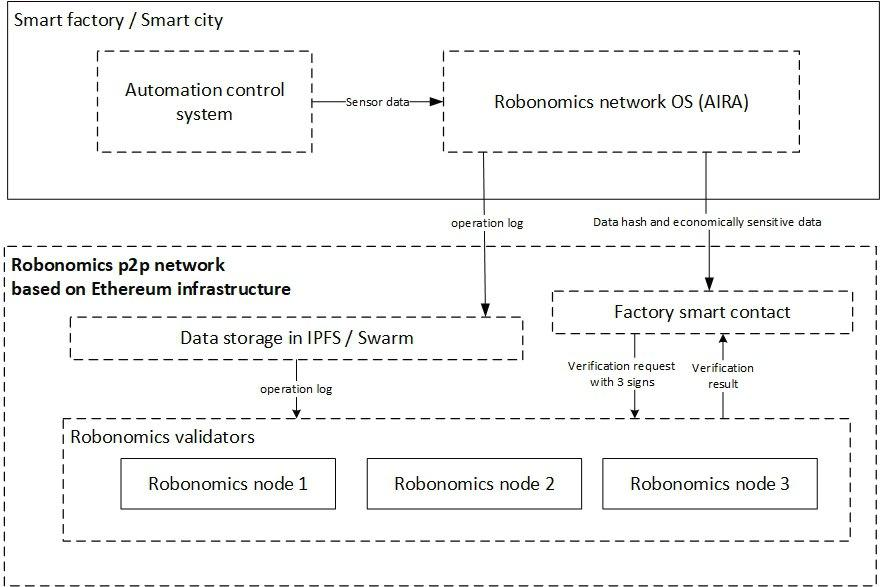
\includegraphics[width=1\textwidth]{app-3.png} 

Робономика способна наблюдать за исполнением обязательств роботов с помощью использования моделей верификации результата работы машины. Для этого необходимо, чтобы в контракте обязательства была указана желаемая в использовании наблюдающая сеть и модель верификации.

Модель поведения в соответствии с framework'ом, применяемым инженером и роботом, является основным элементом свершения работы.  

\subsubsection{Алгоритм работы контракта наблюдателя}

Инициализация контракта происходит так же как и контракта Маяка, на контракт участниками вносится обеспечение, пропорционально которому выдаются квоты на верификацию обязательств.
\begin{enumerate}
	\item В канале результатов появляется сообщение с результатом для обязательства, требующего подтверждение валидатором.
	\item Участник сети наблюдения с маркером подписывает сообщение с результатом и своим решением и отправляет его в канал результатов.
	\item Маяк ловит сообщение с подтверждением валидатора, но поселить его не может N блоков.
	\item Если остальные участники сети наблюдения не согласны с текущим владельцем маркера, они могут опубликовать сообщение в канал результатов со своим решением.
	\item Если по решению не согласному с текущим владельцам маркера набирается BFT, то эта транзакция может быть сразу поселена в контракт обязательства, а текущий владелец маркера лишается квоты.
	\item За верификацию контракта обязательства участнику сети наблюдения переводится комиссия в XRT.
\end{enumerate}

\section{Токен Робономики, XRT}

Задача токена Робономики - обеспечить работу децентрализованной сети по обслуживанию Умных городов и Индустрии 4.0 в инфраструктуре Ethereum. Для достижения данной цели в экономике токена необходимо отразить стимулы выполнения полезной функции сети независимыми провайдерами. Данные стимулы должны быть распределены между эмиссией и комиссией таким образом, чтобы обеспечивать пропускную способность Робономики в Ethereum в зависимости от цены токена XRT, а также мотивировать провайдеров запускать программу Робономики в EVM с данными, предлагаемыми пользователями.

\subsection{Эмиссия за исполнение программы Робономики в Ethereum компьютере}

Существует интересное свойство эмиссии в Bitcoin и Ethereum: вне зависимости от того, есть ли транзакции или нет, блоки всё равно создаются. Данное относительное “безразличие” позволяет гарантировать пропускную способность сети в соответствии с протоколом коммуникации. Эмиссия является ключевым стимулом для майнеров поддерживать заданную пропускную способность, не дожидаясь накопления выгодной суммарной комиссии в блоке.

Представление Робономики как программы для EVM позволяет связать эмиссию XRT токенов с величиной утилизируемого газа как метрикой, являющейся общей для оценки вычисления и сохранения данных любой программы в Ethereum компьютере. Это обеспечит зависимость пропускной способности Робономики в общей инфраструктуре Ethereum от цены токена XRT.

Введем базовую техническую единицу Робономики под названием Wiener (1 XRT = $10^9 Wn$) и определим для нее следующее назначение:
\\
\\
\textit{Emission of 1 wn = 1 gas utilized by Robonomics}
\\
\\
Такая модель означает:
\begin{enumerate}
	\item 1 XRT не равен 1 ETH, так как 1 gas может стоить различное количество wei.
	\item Стоимость 1 wn должна покрывать расходы провайдера на утилизацию 1 единицы gas в Ethereum.
	\item Эмиссию Wn должна иметь возможность выполнять только программа Робономики.
	\item Повышение цены XRT будет способствовать увеличению пропускной способности Робономики.
	\item Общая капитализация XRT может быть больше капитализации ETH, так как несёт в себе дополнительную функцию, кроме утилизации газа в EVM.
\end{enumerate}

Для того, чтобы достичь показателя \textit{Emission of 1 Wn = 1 gas utilized by Robonomics}, мы предлагаем:
\begin{enumerate}
	\item Во время TGE с помощью Голландского аукциона найти начальный множитель эмиссии Wn для покрытия минимально необходимых расходов провайдеров на обеспечения присутствия Робономики в инфраструктуре Ethereum на начальный момент эмиссии. 
	\item Внедрить этап становления сети, в течение которого множитель эмиссии будет алгоритмически снижаться в зависимости от общего объема утилизированного газа в исполнение программы Робономики в EVM.
	\item В последующем обеспечить постоянную эмиссию Wn за каждую утилизированную единицу газа в Ethereum Робономикой. 
\end{enumerate}

\subsubsection{TGE и Голландский аукцион}

В начальный момент запуска Робономики мы предлагаем выпустить 10,000,000 XRT, из которых от 5\% до 77\% будет доступно для голландского аукциона. Мы ставим цель в  N ETH для сбора средств на счет специально создаваемого Фонда экономики роботов, который будет развивать базовую концепцию представления КФС как экономически автономных агентов. Чем больше моделей экономически автономных агентов, доступных для использования в любой точке планеты, тем выше вероятность задействования Робономики в целом.

В результате аукциона все участники получат токены по минимально возможной цене, а Робономика получит начальное соотношение XRT к ETH. Совместив эти данные со статистикой текущей цены газа, мы сможем определить начальный множитель эмиссии на период становления Робономики в инфраструктуре Ethereum, чтобы покрывать расходы провайдеров по конкурентной цене при условии естественно меньшей капитализации Робономики относительно Ethereum на начальном этапе. По нашим расчетам на весну 2018 года минимальной конкурентной ценой в сети Ethereum является цена в 2 gwei за 1 gas. 


\subsubsection{Становление}

Период становления Робономики в инфраструктуре Ethereum мы разделяем на 5 эпох, каждая из которых оценена статистически в суммарном объеме утилизированного газа в Ethereum. По своему завершению эпоха алгоритмически снижает множитель эмиссии таким образом, чтобы по завершению периода становления выполнялось условие:
\\
\\
\textit{Emission of 1 wn = 1 gas utilized by Robonomics}
\\
\\
То есть множитель должен снизиться до единицы, исчезнуть в прошлом.
\\
\\
Ниже приводится таблица параметров пяти эпох становления Робономики:
\\
\\
\begin{tabular}{ |l |l |l |l}
 \textbf{Epoch} & \textbf{Utilized gas} & \textbf{E(i), Wn} & \textbf{E(i), XRT} \\ 
 \hline
 1 &  3,47E+12 & 2,08E+13 & 2,08E+06 \\ 
 2 &  3,47E+12 & 1,39E+13 & 1,39E+06 \\ 
 3 &  3,47E+12 & 9,26E+12 & 9,26E+05 \\ 
 4 &  3,47E+12 & 6,17E+12 & 6,17E+05 \\ 
 5 &  3,47E+12 & 4,12E+12 & 4,12E+05 \\ 
 Total &  1,74E+13 & 5,43E+13 & 5,43E+06 \\ 
\end{tabular}

Нами заложен объем газа в блоке как постоянная величина, так как предсказать его рост на сегодня фактически невозможно. Соответственно, мы можем только судить о том, что прохождение каждой эпохи означает утилизацию процентного количества газа по данным о размере блока в Ethereum на период весны 2018 года. То есть при завершении пятой эпохи мы можем говорить о том, что Робономика справилась с показателем в один годовой объема газа, который был доступен в сети Ethereum весной 2018 году. В любом случае данной статистики будет достаточно для объективной оценки роста Робономики относительно момента проведения TGE в 2018 году.

\subsubsection{Дальнейшая эмиссия}

После прохождения стадии становления Робономика выйдет на постоянную величину эмиссии, количественно равную желаемому показателю Emission of 1 wn = 1 gas utilized by Robonomics.

Данная линейная зависимость будет способствовать обеспечению минимальной пропускной способности, которую способны дать провайдеры после выравнивания капитализации Робономики без наличия комиссии.

\subsection{Комиссии за запуск программы Робономика в Ethereum инфраструктуре}

Первое отличие исполнения программы Робономики в EVM с настоящими участниками от симуляции заключается в неопределенном промежутке времени с момента создания контрактного обязательства для КФС до момента отправки результата работы и финализации выполнения программы на основании этой транзакции. Отсюда следует, что КФС должны быть заинтересованы в оплате комиссии сети, покрывающей расходы провайдера на работу в информационных каналах для поиска согласованных спроса с предложением КФС, а также издержек на поселение транзакции по созданию контрактного обязательства в Ethereum Blockchain. 

\subsection{Дополнительные задачи XRT токена}
\subsubsection{Наблюдающие сети существуют за счет комиссии пользователей}

Мотивировать провайдеров финализировать выполнение программы Робономики с учетом наблюдающей сети или без нет необходимости. Любой провайдер с удовольствием финализирует выполнение программы Робономики ради эмиссии.

Таким образом, комиссия пользователя услуги КФС может быть использована исключительно для оплаты проверки результатов исполнения модели поведения КФС.

\subsubsection{XRT на счету маяков как механизм доверия к Робономике}

В нулевой момент существования Робономики провайдеры будут заинтересованы в создании “индивидуальных” маяков с минимальной ставкой XRT, в формате обеспечения, на контракт маяка. С момента появления спроса и предложения в Робономике интерес к работе на конкретном маяке будет тем выше, чем больше суммарная комиссия, которую может получить провайдер с информационного канала, обслуживаемого маяком. Со временем провайдеры начнут консолидироваться вокруг тех маяков, где доля обеспечения провайдера, размещенная на контракте маяка, будет давать достаточное время работы, чтобы получить дополнительную выгоду. 

В конечном результате, чем выше будет суммарная комиссия с определенных информационных каналов, тем большую долю XRT провайдеры готовы будут заморозить. Чем больше объем замороженных на маяке средств, тем выше доверие остальных участников к работе данного маяка и к Робономике в целом.  

\subsubsection{XRT как количественное отражение капитала сети}

Капитал Робономики есть не что иное, как отражение ценности сети, использующей Ethereum инфраструктуру для построения коммуникации с экономически автономными КФС. 

Рост капитала такой сети, с одной стороны, будет связан с ростом количества людей в обществе, принимающих идею представления КФС как автономных экономических агентов, а с другой - взглядом на Ethereum как на инфраструктуру, подходящую для экономически значимой коммуникации по академическим и промышленным стандартам автоматизации.

\subsubsection{Рынок кибернетики}

В долгосрочной перспективе, являясь токеном необходимым КФС для заключения контрактных обязательств и верификации их результата, XRT превратится во внутреннюю валюту рынка контрактных обязательств роботов для роботов. Рынок, в котором каждое исполнение программы будет зациклено на исполнение программы.

\subsubsection{Выводы о движении XRT в Робономике}

Итак, мы получаем, что эмиссия XRT призвана поддерживать постоянную готовность Робономики выполнить коммуникацию с КФС как с автономным экономическим агентом в инфраструктуре Ethereum. Комиссии создают стимул для использования пользовательских данных в исполнении программы Робономики провайдерами.

\subsubsection{Denomination }
\begin{tabular}{ l |l |l |l |l}
 Значение &  $1$ & $10^3$ & $10^6$  & $10^9$ \\ 
 \hline
 Наименование в Robonomics platform &  wiener & coase  & glushkov & robonomics token\\ 
\end{tabular}

\section{Описание работы Робономики}
\subsection{Предложение новой модели поведения инженером}

\begin{wrapfigure}{l}{0.30\textwidth} %this figure will be at the right
    \centering
    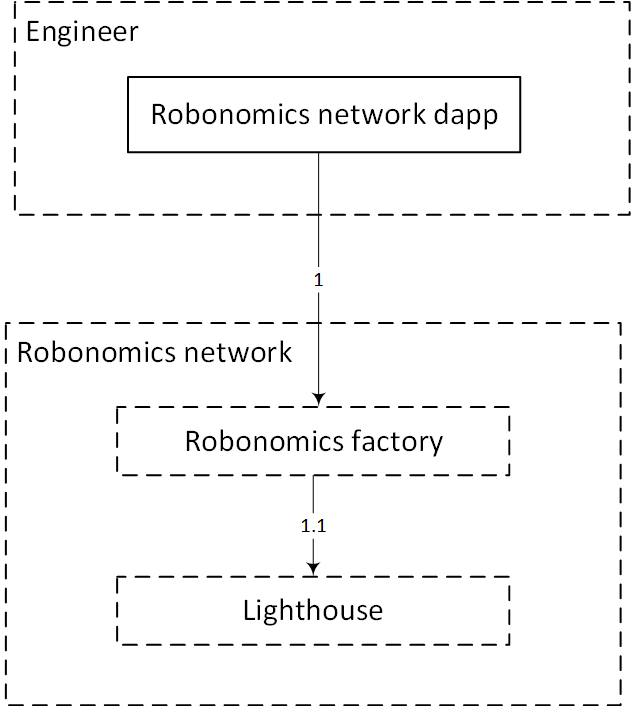
\includegraphics[width=0.30\textwidth]{step-by-step-1.png}
\end{wrapfigure}

Lighthouse - автономный рабочий процесс, позволяющий распределить время работы провайдеров, обслуживающих конкретный широковещательный канал.

Robonomics factory - автономный рабочий процесс, позволяющий создать новый маяк или обязательство, используя соответствующие библиотеки, сохраненные в Ethereum Blockchain.

Организации, создающие кибер-физические системы, могут быть заинтересованы в представлении их роботов как сервисов, способных учитывать собственную экономику: от получения технических и финансовых параметров перед оказанием услуги до самостоятельного обеспечения своей работы необходимыми ресурсами и обслуживанием за счет средств, находящихся под управлением КФС.

Для подобных задач инженер может создать ROS-совместимую модель поведения, которую он хочет предложить использовать владельцам кибер-физических систем, чтобы их роботы начали работать как экономически автономная система.

Инженер с помощью dapp подключается к сети Робономики и отправляет в Ethereum транзакцию (1), содержащую хэш модели поведения ROS-совместимой кибер-физической системы.

На основе транзакции от инженера (1) происходит внутренний вызов (1.1) создания нового автономного рабочего процесса Маяка в Ethereum Blockchain.

\subsection{Начало работы провайдера сети Робономики}

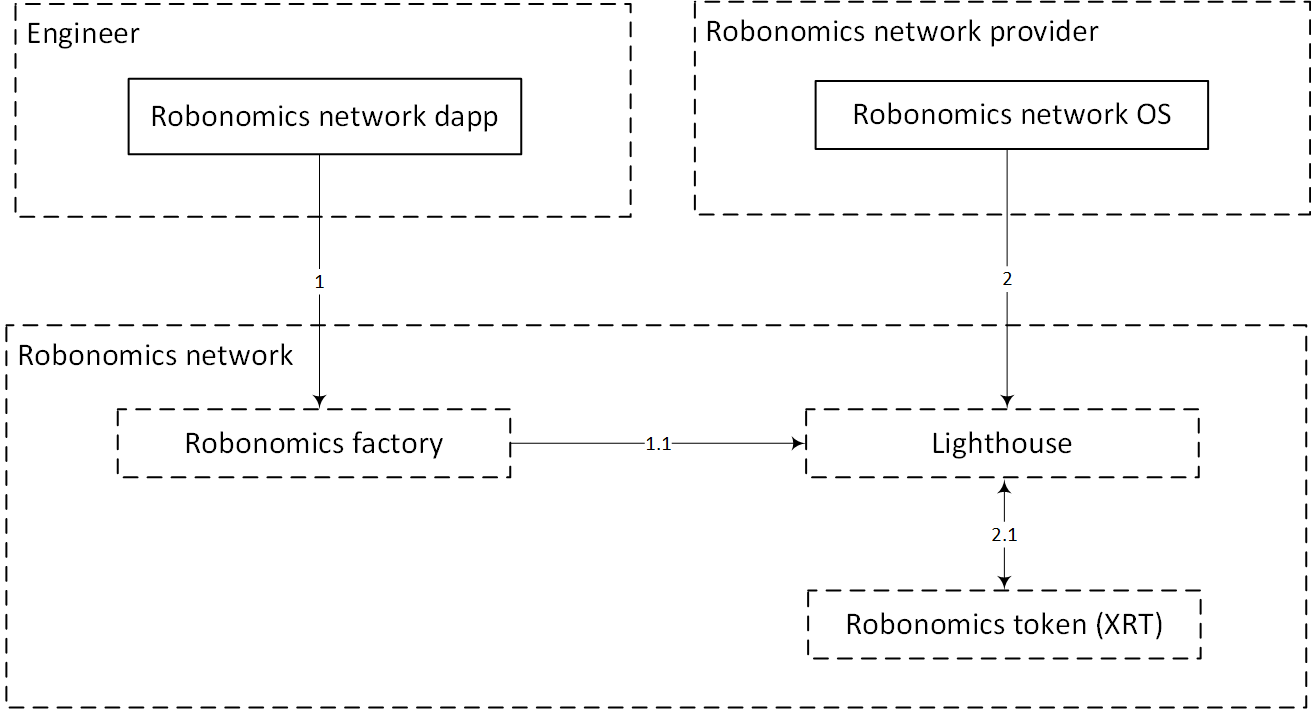
\includegraphics[width=1\textwidth]{step-by-step-2.png}

Провайдер сети Робономики отправляет транзакцию (2) к созданному (1) маяку, передав некоторое количество токенов XRT (2.1) как обеспечение, используемое в распределении времени работы на маяке среди провайдеров.

\subsection{Начало работы кибер-физической системы как сервиса}

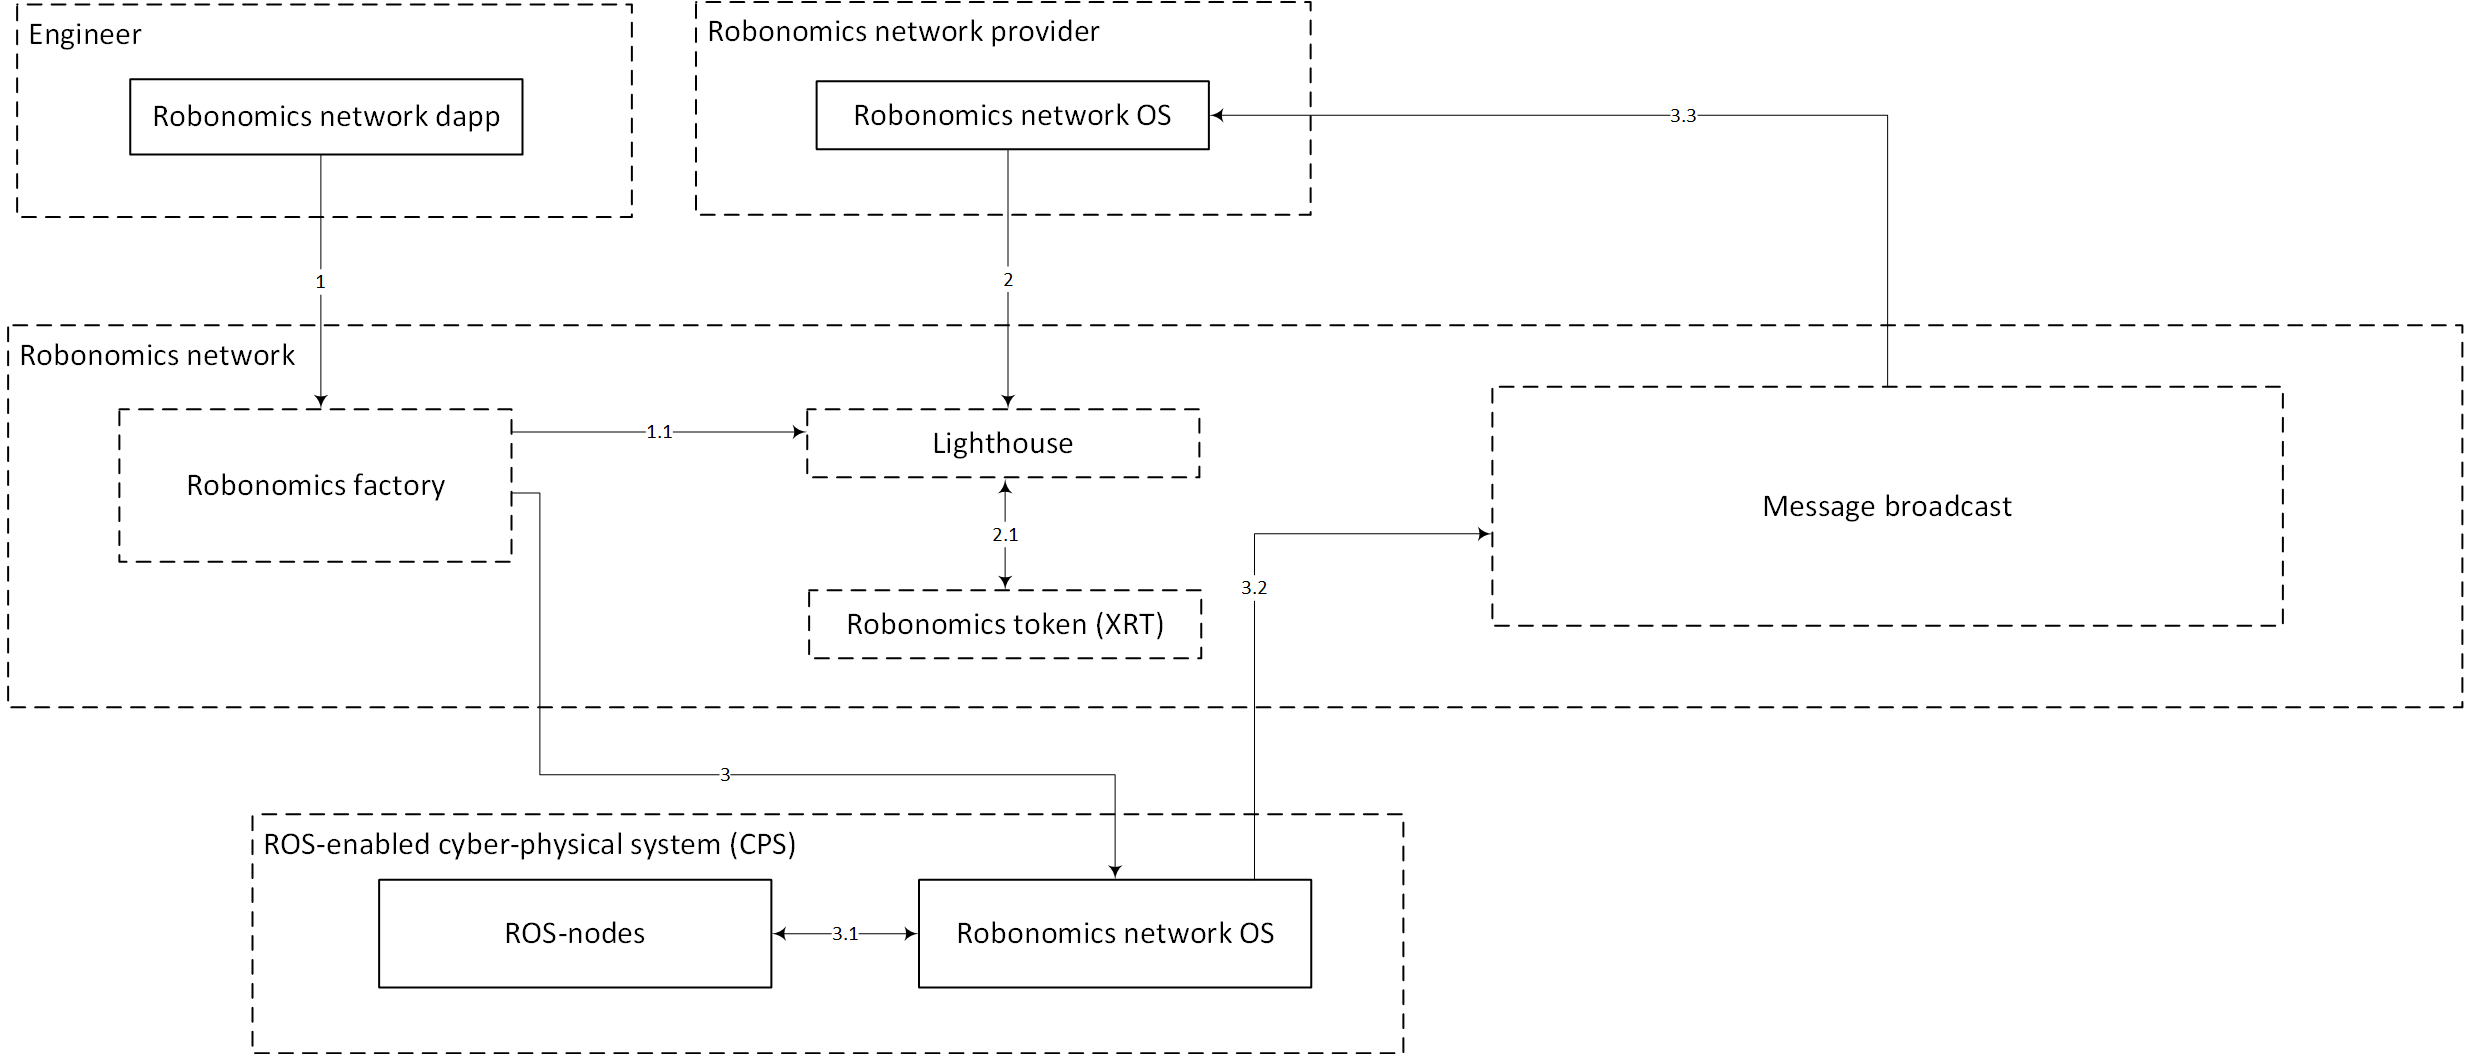
\includegraphics[width=1\textwidth]{step-by-step-3.png}

Robonomics network OS получает список созданных маяков от фабрики Робономики (3). Используя информацию из описания маяков и опрашивая свои узлы (3.1), КФС начинает публиковать свои предложения об оказании услуг в каналы широковещательной рассылки Робономики (3.2). 

Провайдер сети Робономики получает сообщение через канал широковещательной рассылки о появлении нового предложения от КФС (3.3).

\subsection{Появление пользователя в сети Робономики}

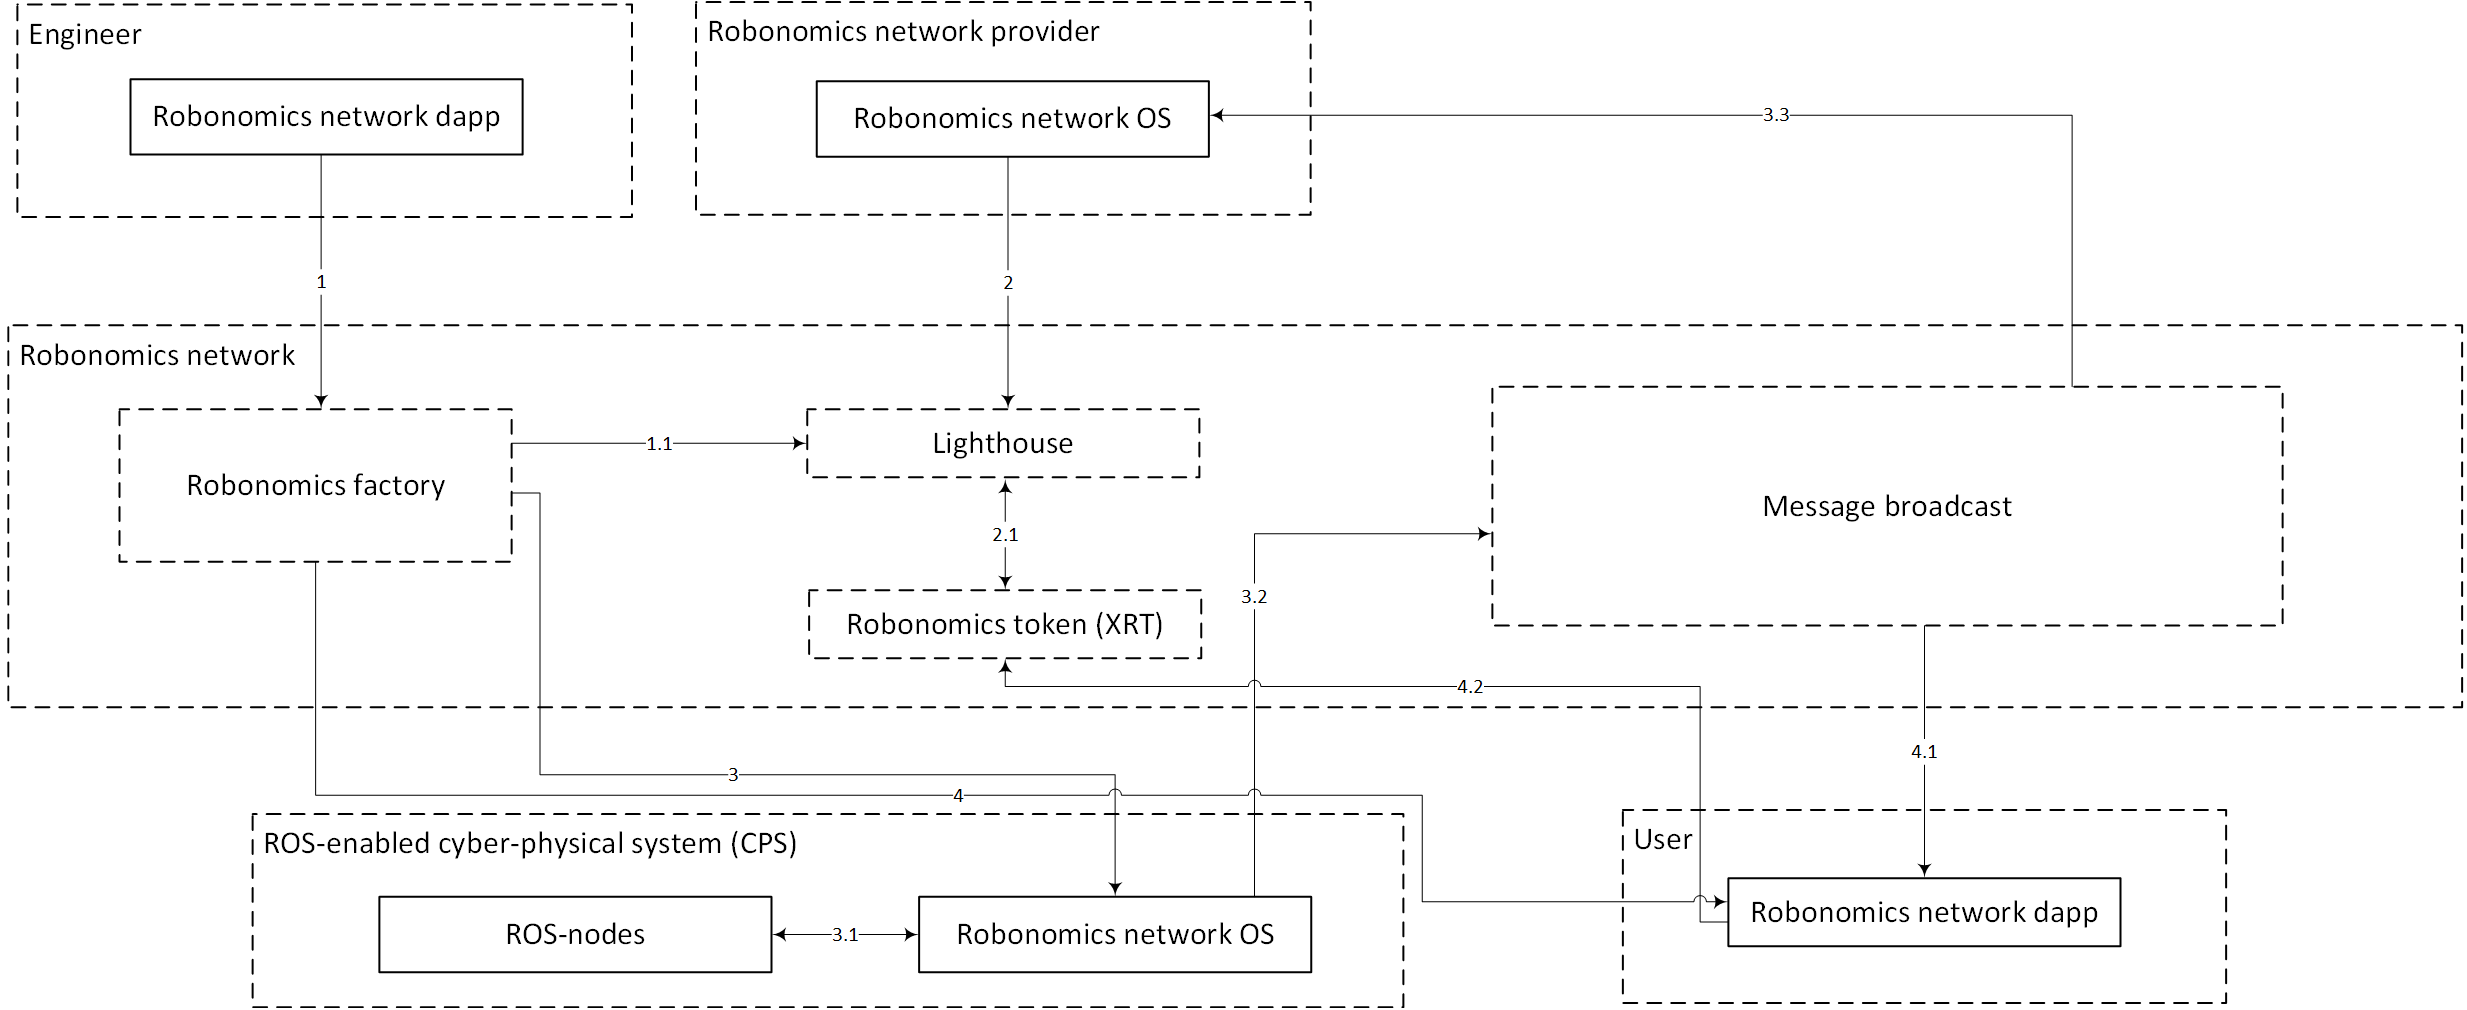
\includegraphics[width=1\textwidth]{step-by-step-4.png} 

Пользователь получает список широковещательных каналов Робономики (4) с помощью dapp и начинает слушать сообщения в данных каналах (4.1). Пользователь, убедившись, что в сети Робономики есть интересующая его услуга от КФС (3.2), отправляет транзакцию в Ethereum Blockchain для разрешения снятия XRT токенов автономным рабочим процессом фабрики Робономики (4.2).

\subsection{Создание обязательства на исполнение сервиса кибер-физической системой}

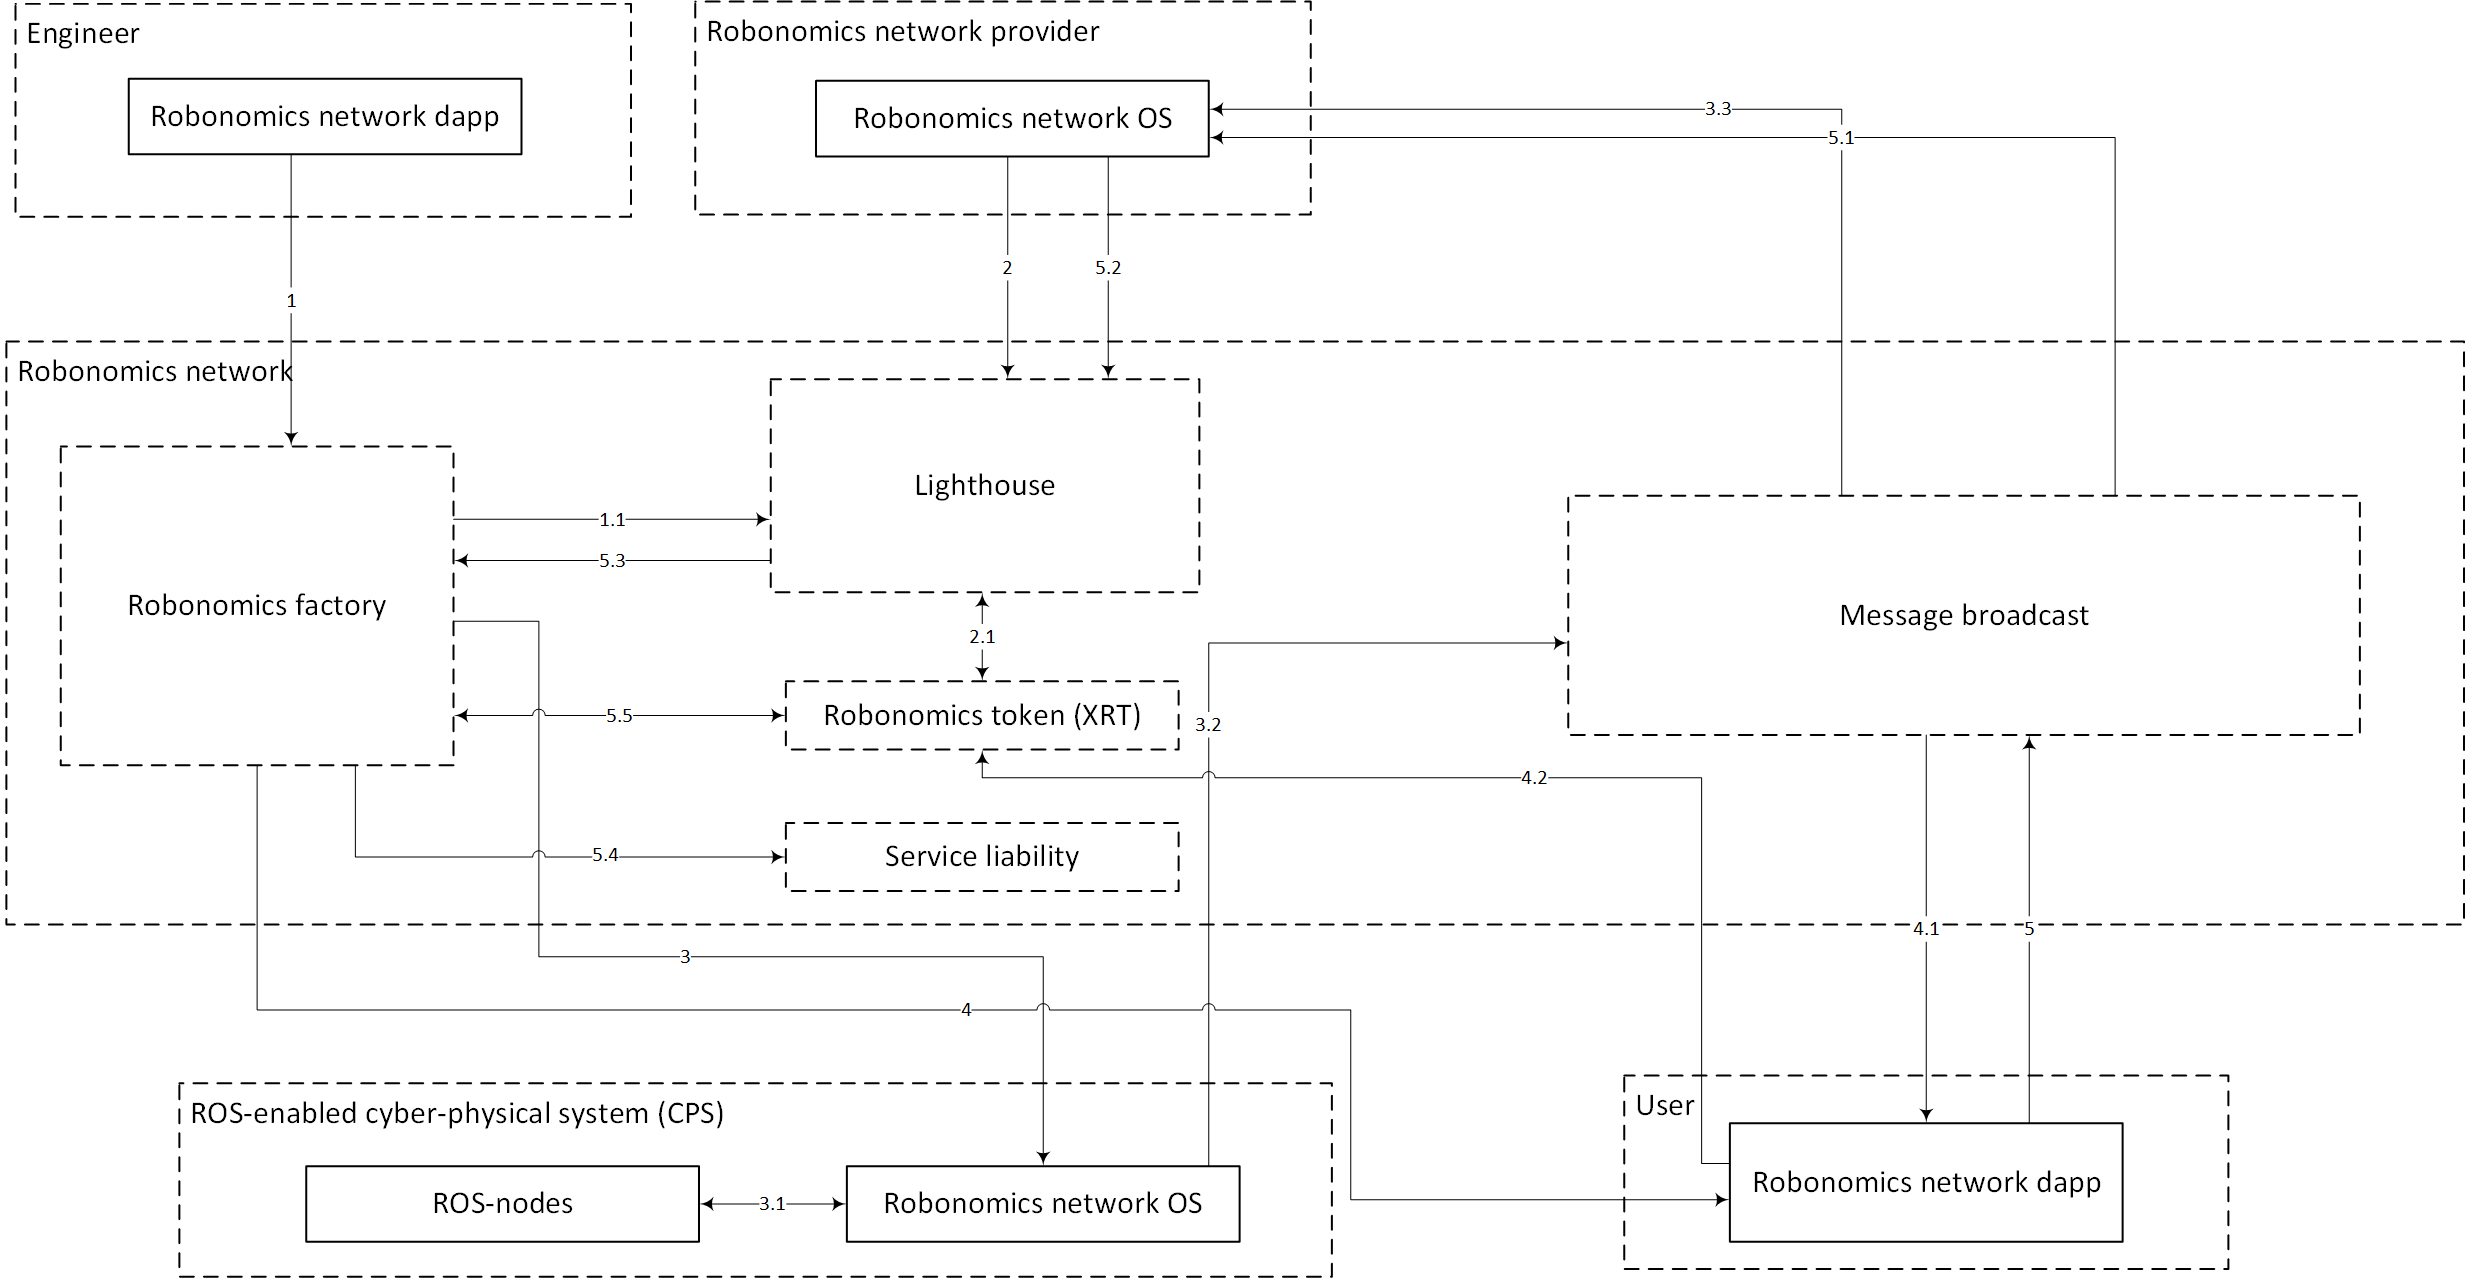
\includegraphics[width=1\textwidth]{step-by-step-5.png} 

Пользователь, имея достаточное количество XRT токенов для отправки спроса на интересующую его услугу, может отправить в широковещательную рассылку сообщение о своем спросе (5) на ранее опубликованную КФС услугу (4.2).

Провайдер сети Робономики, получив сообщение пользователя (5.1) и имея локально сохраненное сообщение от КФС (3.3), которые согласованы по значению хэша от модели поведения ROS-совместимой КФС и стоимости оказываемой услуги, обращается к автономному рабочему процессу Маяка (5.2), передавая отложенные подписи обеих сторон.

Маяк обращается к фабрике Робономики (5.3) для создания обязательства на оказание услуги (5.4), фабрика же, создав контракт обязательства и зная его адрес в Ethereum Blockchain, обращается к контракту XRT (5.5) для:
\begin{enumerate}
	\item Перевода стоимости оказываемой услуги со счёта пользователя (4.2) на счет контракта;
	\item Эмиссии XRT токенов на счет контракта в объеме общего количества, требуемого для утилизации газа, умноженного на стартовый фактор, в Ethereum Blockchain.
\end{enumerate}

\subsection{Исполнение обязательства кибер-физической системой}

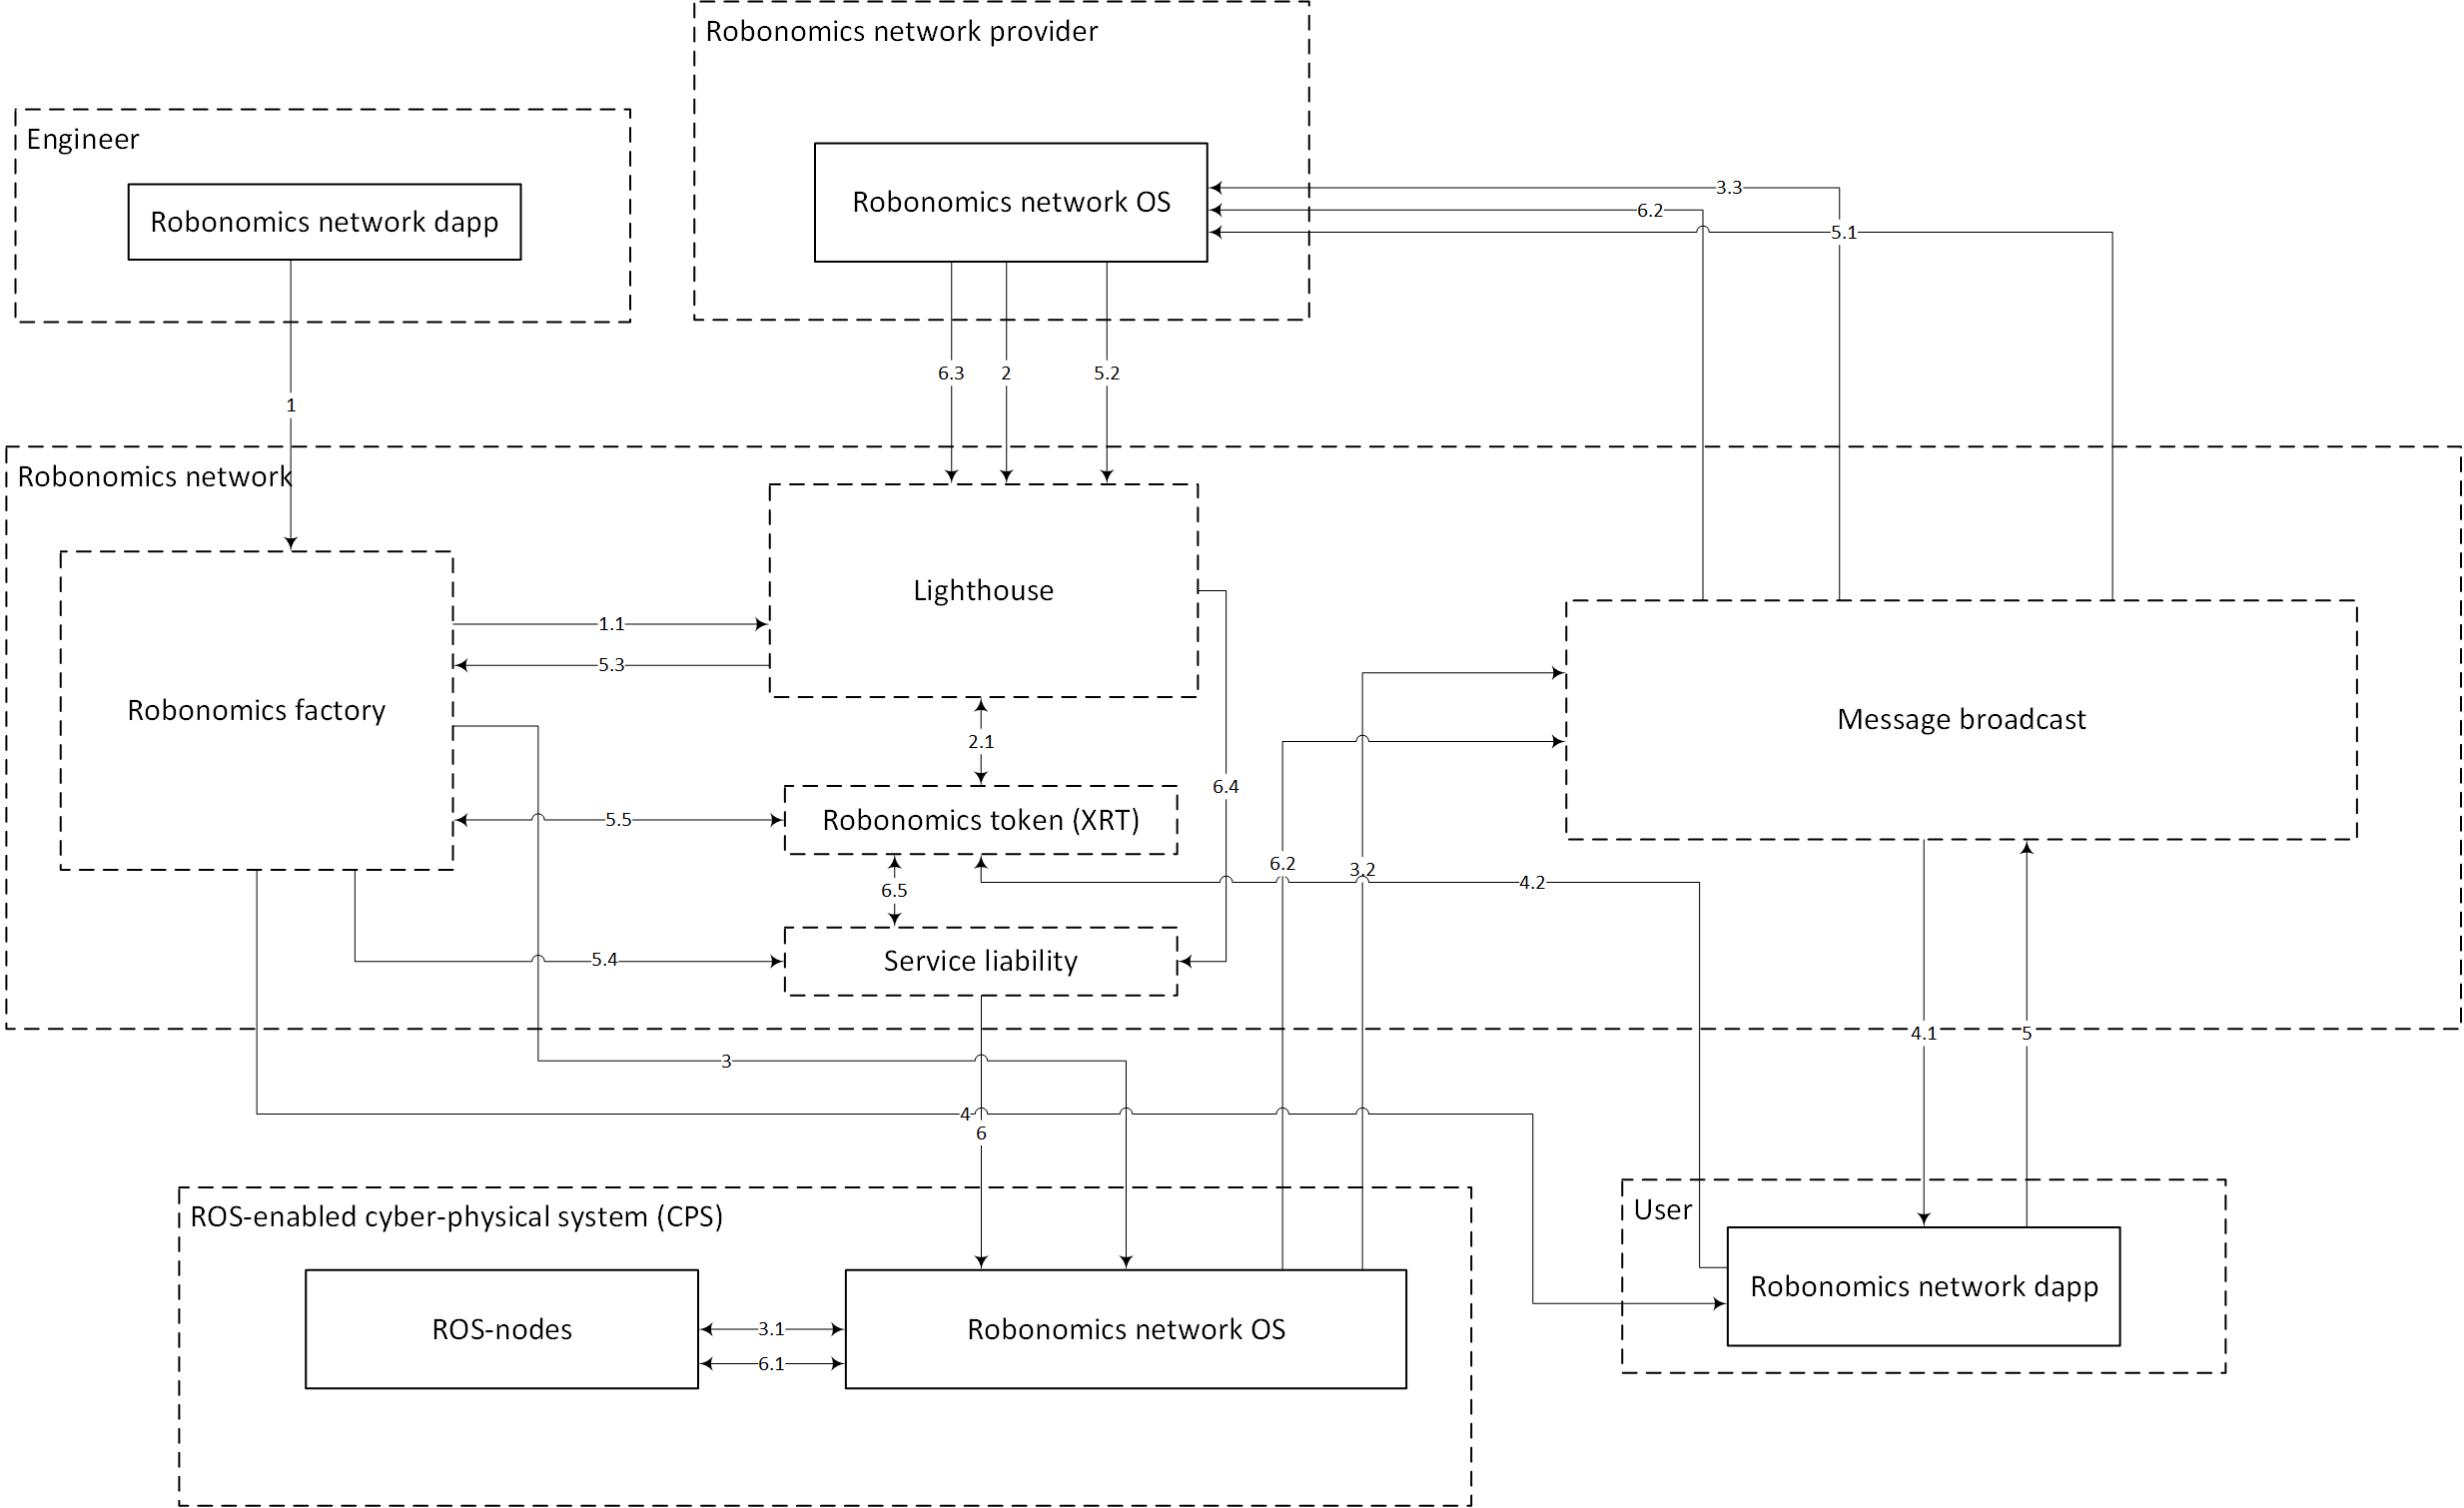
\includegraphics[width=1\textwidth]{step-by-step-6.png} 

С помощью Robonomics network OS кибер-физическая система получает уведомление о созданном для нее контракте обязательства, в котором можно узнать хэш модели поведения и хэш параметров (переменных) модели поведения (6). 

Загрузив на исполнение модель поведения и параметры (6.1), КФС с помощью ROS-bag приступает к исполнению полученного обязательства.

Во время исполнения КФС формирует лог операций и после завершения работы отправляет его хэш в информационный канал Робономики, обслуживающий данную модель поведения (6.2).

Провайдер сети Робономики получает хэш лога (6.2) и отправляет транзакцию о выполнении обязательства со стороны КФС (6.3) в Ethereum Blockchain к Маяку (6.3). Маяк создает внутреннюю транзакцию к соответствующему обязательству на выполнение услуги и записывает туда хэш лога операций КФС (6.4). После этого с контракта обязательства высвобождается вознаграждение за оказанную услугу на адрес КФС, а также эмиссия XRT на адрес того провайдера, который отправил транзакцию в Маяк.

\section{Приложения платформы Робономики}

\subsection{Создание доверия к продукции умных городов и умных фабрик}

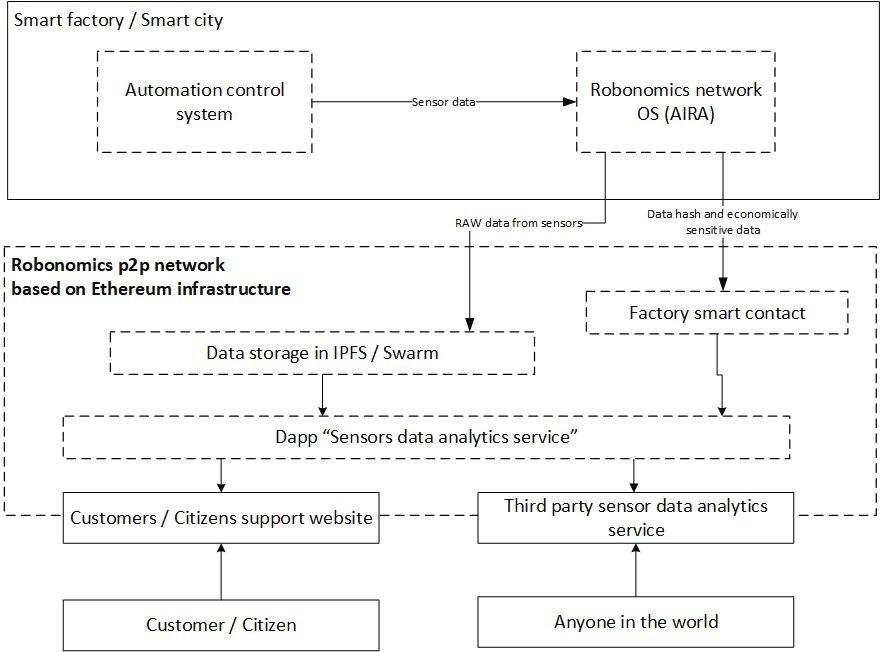
\includegraphics[width=1\textwidth]{app-1.png} 

Вопрос доверия между потребителем и умной фабрикой заключается в том, как потребитель может быть уверен в качестве продукта, произведенного умной фабрикой. Продукты в магазине могут быть очень похожи, но иметь очень разную историю происхождения. Мы предлагаем протоколировать технологический процесс, размещая его в децентрализованной сети. Хеш от лога операций КФС сохраняется в блокчейн, наделяя историю продукта свойством иммутабельности. Потребитель уверен в продукте, так как его история не может быть изменена в будущем. 

\url{https://github.com/airalab/robonomics_comm/blob/master/robonomics_liability/src/robonomics_liability/executor.py#L50}

Здесь происходит сбор и аккумулирование данных производственного процесса в момент исполнения обязательства умной фабрикой.


\begin{python}
 {
	msg.result = self.ipfs.add(result_file)['Hash']
	self.complete.publish(msg)
  }
\end{python}


Лог операций сохраняется в IPFS сеть, а его хеш публикуется в контракт обязательства и не может быть изменен в будущем.

\subsection{Запуск умной фабрики пользователем}

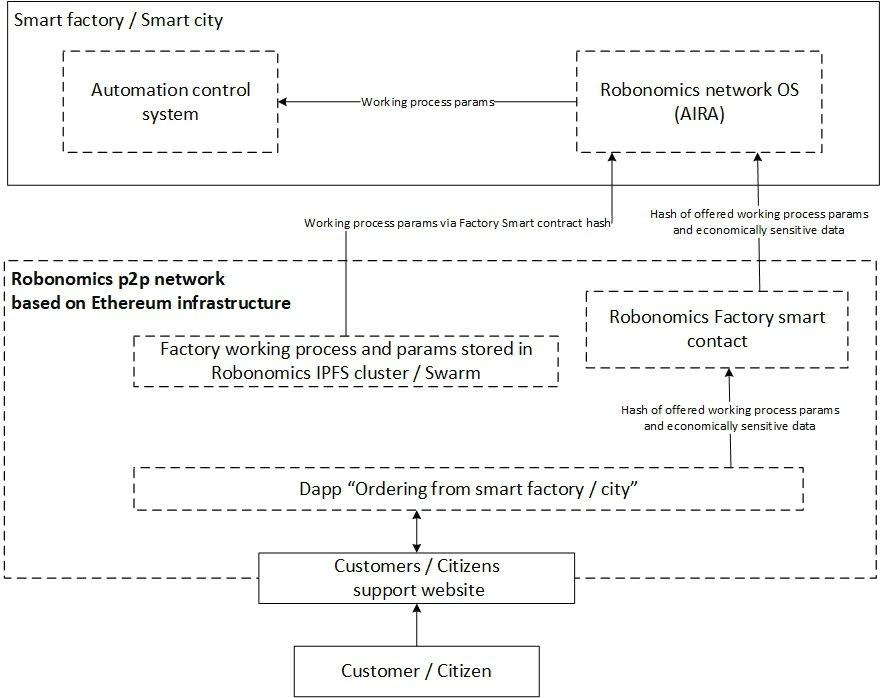
\includegraphics[width=1\textwidth]{app-2.png} 

Проблема доступа к фабрике как к сервису для потребителя заключается в том, чтобы устранить посредника, который как-либо может повлиять на их взаимодействие. Умный контракт является подходящим объектом.

\url{https://github.com/airalab/robonomics_comm/blob/master/robonomics_liability/src/robonomics_liability/executor.py#L34}

Здесь умная фабрика слушает события от фабрики умных контрактов, принимая обязательства, в которых она указана как исполнитель.

\begin{python}
rospy.logdebug('Getting objective %s...', msg.objective)
self.ipfs.get(msg.objective)

player = Player(msg.objective)
player.start()
\end{python}

Когда обязательство взято, умная фабрика начинает его исполнение, скачивая параметры обязательства из IPFS и воспроизводя их последовательность локально.

\subsection{Управление экономикой роботов с помощью капитала}

Представим множество экономически самостоятельных киберфизических систем или просто роботов как вектор (R), а капитал (инвестиции) — как вектор (K). Здесь вектор $ R = {R_i, i=\overline{1,n}}$, где $R_i$ — количество роботов на рынке i, n — количество рассматриваемых рынков. А вектор $ K = {K_j, j=\overline{1,n}} $, где  $K_j$ — инвестиции в j-й рынок. Сформулируем описание модели пропорционального капиталу распределения роботов на рынке следующим образом:
\[
R'[k] = K[k] *  \frac{ \sum R_i[k]}{ \sum K_i[k] }
\]
\[
e[k] = R'[k] - R[k-1] ;
\]
Здесь:
\begin{itemize}
\item $R'[k]$ — желаемое распределение роботов на рынках [штук];
\item $R[k-1]$ — количество роботов, уже присутствующих на данном рынке капитала;
\item e — вектор ошибок распределения (отклонение от желаемого значения распределения) [штук];
\item $i \in \overline{1,n}$ - индекс рынка;
\item k - шаг дискретного времени;
\item $\sum R_i[k] $ - количество роботов на всех рассматриваемых рынках на шаге k;
\item $\sum K_i[k] $ - объём инвестиций в рассматриваемые рынки на шаге k.
\end{itemize}

Исходя из выше описанного, можно сформулировать закон управления экономикой роботов следующим образом:

Каждый робот должен стремиться к участию на том рынке, где ошибка распределения выше \cite{2017}.

При включении очередного робота в экономику рынок для размещения своего предложения этим роботом выбирается из равенства:

$ i = maxi(e[k])$, что приводит к $ e_i[k] \rightarrow 0 $.

Здесь  $ maxi(e) $ - индекс максимального элемента вектора отклонения. 

\subsubsection{Референсная имплементация}

Реализация алгоритма управления экономикой роботов содержится в пакете robonomics\_control

\url{https://github.com/airalab/robonomics_comm/tree/master/robonomics_control}. 

Здесь алгоритм линейного распределения основан на информации из умного контракта о распределении капитала и информации с рынков о лотах от кибер-физических систем. 

\url{https://github.com/airalab/robonomics_comm/blob/master/robonomics_control/src/robonomics_control/distribution.py}

\subsection{Токенизированные ценности на основе труда робота}

Рассмотрим сценарий выпуска карбоновых единиц сенсором в умном городе. Сенсор наделяется правом эмиссии токена карбоновых единиц, если загрязнение воздуха ниже некоторого значения.

Пусть сенсор в результате обязательства по измерению степени загрязнения воздуха совместно с результатами присылает количество освобожденных карбоновых единиц. Расширим стандартный контракт обязательства методом, принимающим совместно с результатом работы количество единиц для эмиссии.
\begin{lstlisting}
function setResult(bytes32 _result, uint256 _emission);
\end{lstlisting}


Таким образом, значения для выпуска карбоновых единиц сохраняются в контракте обязательства. И при условии, что сеть наблюдателей подтвердит корректность измерений сенсора, по контракту обязательства будет эмиссировано соответствующее число токенов.

\begin{lstlisting}
function confirm() {
  ... 
  carbonToken.emission(emission);
}
\end{lstlisting}

Здесь важно, что контракт обязательства добавляется в группу, которой доступна эмиссия токена, совершенная фабрикой на этапе создания. Тогда фабрика контрактов обязательств обязана обладать информацией о соответствии заданной модели поведения такому токену, который может быть эмиссирован при успешном исполнении обязательства.

\section{Масштабируемость}

Робономика проектируется для представления таких крупных кибер физических систем, как, например, целая фабрика или город. Действующая на сегодня пропускная способность сети Ethereum является достаточной, чтобы обеспечить исполнения более 1,000 контрактных обязательств в сутки. К примеру, этого достаточно для:
Организации ежедневного прямого заказа покупателями автомобилей на сайтах нескольких автоконцернов таких, как BMW, Porsche, Avtovaz.
Регистрации регулярных маршрутов для беспилотной логистики текущих промышленных зон мира.
Ежедневной публикации отчетов о состоянии окружающей среды от сенсорных сетей всех городов мира с населением свыше 1,000,000 человек.

\section{Сегмент Робономики в сети Ethereum}

С внедрением возможности создать собственный сегмент в сети Ethereum Робономика может выделиться в сегмент с повышенной пропускной способностью, а также позволить многократно повысить количество возможных исполнений роботами контрактных обязательств для того, чтобы покрыть запрос всей Индустрии 4.0 со стоимостью сделок свыше 1,000 \$.

\section{Заключение}

Платформа Робономики ставит своей целью решение социально-экономических задач тотальной роботизации массового производства, жизни городов и логистики. Основным применением платформы можно считать задачи, связанные с созданием доверия к услугам и продукции умных городов и фабрик, предоставления прямого доступа пользователей к автономным кибер-физическим системам и управление мультиагентными системами с помощью капитала. 

Платформа Робономики позволит расширить возможности инфраструктуры сети Ethereum с целью ее использования в таких областях, как Индустрия 4.0, IoT, умные города.
\newpage
\printbibliography
\newpage
\section*{Приложение 1: Вопросы на стыке робототехники и экономической теории}

Тотальная роботизация. Приход роботов в жизнь каждого человека неизбежен. Машины способны выполнять недоступные человеку задачи, они эффективнее во многих видах операционной деятельности и экономят человеку время в повседневных делах уже сегодня.

Развитие робототехники достигло такого этапа, на котором появились задачи коммуникации между физически или логически выделенными автономными агентами - роботами, имеющими право решать, какие действия являются целесообразными в рамках их существования \cite{Kapitonov2017Blockchain-basedUAVs}. Технологии, находящие применение в мире машин, расширяют доступный роботу набор принимаемых решений, что с каждым разом повышает уровень его автономности.

Наиболее ярко задачи коммуникации автономных роботов раскрываются в таких идеях, как Индустрия 4.0 и Интернет вещей. Ниже приведены наиболее значимые на взгляд авторов данной работы вопросы участия автономных роботов в жизни человека:    

\begin{itemize}
	\item Как обеспечить доверие к продукции роботизированных сервисов?
	\item Как обеспечить передачу права собственности потребителю, если в процессе производства и логистики не участвует человек?  
	\item Как полностью автоматизированному предприятию за окном понять изменяющиеся потребности человека?
	\item Как обеспечить прямое взаимодействие между роботами двух различных корпораций?
	\item Как взимать налоги с деятельности роботов и что считать отдельной роботизированной единицей?  
\end{itemize}

Варианты ответов на данные вопросы влекут за собой различные риски повышения нестабильности и возможного коллапса мировой системы - это вызов на пути построения общества, в котором нет места рабскому труду человека.

\section*{Приложение 2: Дистрибутив AIRA}

Опорной (референсной) реализацией ОС Робономики является проект AIRA (https://github.com/airalab/aira). Дистрибутив AIRA основан на дистрибутиве NixOS GNU/Linux и развивается открытым сообществом, в которое входят разработчики Airalab.

\paragraph{NixOS}

Основу дистрибутива составляет ответвление от базы пакетов nixpkgs (\url{https://github.com/airalab/airalab-channels}), в которое командой Airalab добавлены важные пакеты инфраструктуры Ethereum (такие, как parity, web3.py); поддержка Robot Operating System, а также фундаментальные пакеты коммуникационного стека сети Робономики: robonomics\_market, robonomics\_liability.

\paragraph{ROS}

Минимальная поддержка ROS обеспечена в рамках метапакета ros\_comm с задействованием необходимого базового стека ПО для сериализации и обмена сообщениями между участниками сети ROS, вызова сервисов и интеграции в единое пространство имен rosgraph.
	
На базе дистрибутива формируются установочные образы стендов Фабрики экспериментов (\url{https://aira.life/cases/}): Game of trains, Industry 4.0 in use.

\section*{Приложение 3: Внешнее API AIRA}

\begin{tabular}{ l |l}
	/market/incoming/ask & Входящие сообщения со спросом из информационного канала. \\
	/market/incoming/bid & Входящие сообщения с предложением из информационного канала. \\
	/market/sending/ask & Исходящие сообщения спроса в информационный канал. \\
	/market/sending/bid & Исходящие сообщения предложения в информационный канал. \\
	/market/signing/ask & Исходящие сообщения спроса на подпись. \\
	/market/signing/bid & Исходящие сообщения предложения на подпись. \\
\end{tabular}

\section*{Приложение 4: Программа ДАО}

\paragraph{Представление экономики роботов, как программы для децентрализованного компьютера Ethereum}

Чтобы получить децентрализованную службу, необходим децентрализованный компьютер и программа, адаптированная под его специфику. Рабочие процессы, позволяющие задействовать инфраструктуру сети Ethereum для Умных городов и Индустрии 4.0, могут быть представлены в виде программы для компьютера Ethereum. 

Представим, что у нас есть программа с названием “Сеть экономики роботов”, мы загружаем её в Ethereum Blockchain на хранение. Программа позволяет участникам инфраструктуры Ethereum включить  “Сеть экономики роботов” на своих виртуальных машинах и тем самым организовать новую службу в децентрализованной среде, выступив её провайдером.

\paragraph{Представление экономики роботов, как ДАО}

Автономные рабочие процессы и их исполнители образуют ДАО. Исполнитель не может повлиять на работу ДАО, он может лишь следовать инструкциям. Экономические стимулы должны поддерживать интерес исполнителя для полного выполнения рабочего процесса. Рабочий процесс не может быть изменен без последствий в Ethereum Blockchain.

\end{document}
